\documentclass[tikz,border=8pt]{standalone}

\usepackage{amsmath}
\usetikzlibrary{arrows.meta,calc}

\begin{document}
	
	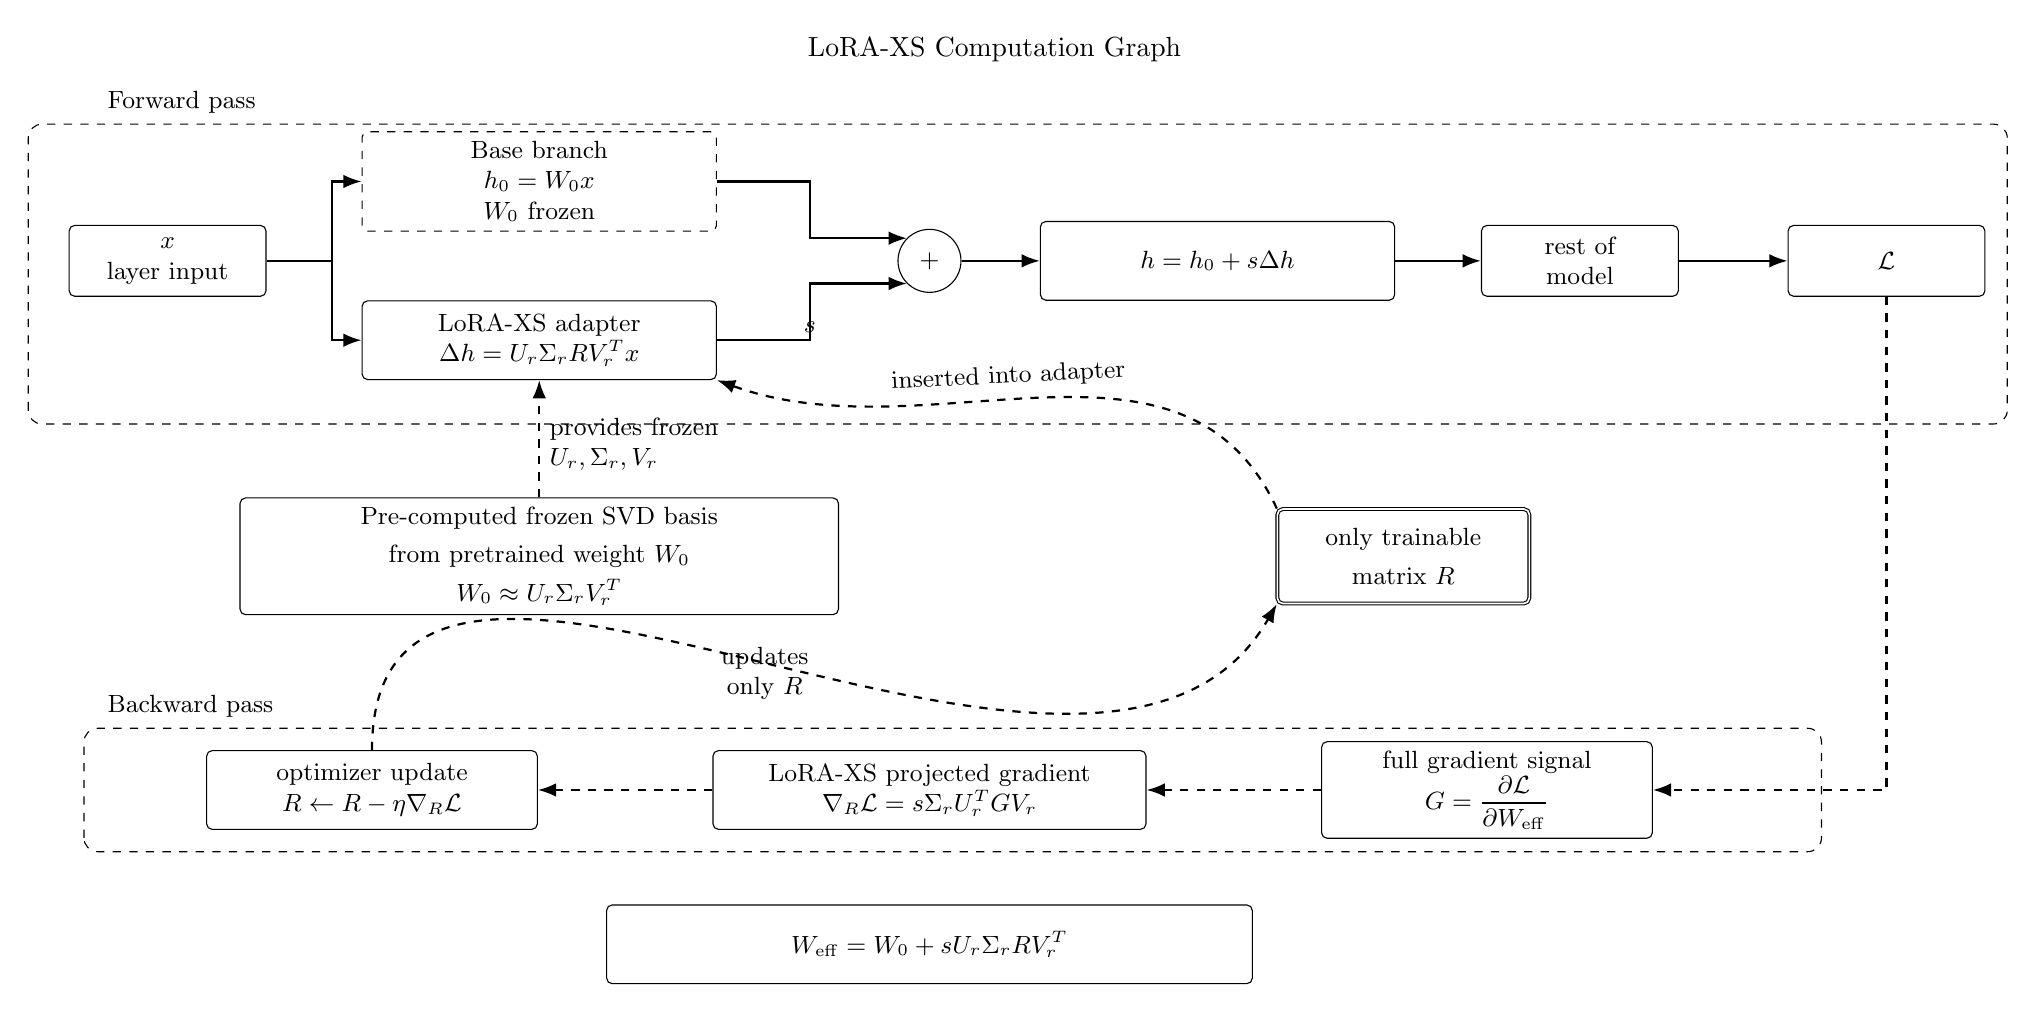
\begin{tikzpicture}[
		x=1.18cm,
		y=1.12cm,
		font=\small,
		>=Latex,
		box/.style={draw,rounded corners=2pt,align=center,minimum width=25mm,minimum height=9mm,fill=white},
		wide/.style={draw,rounded corners=2pt,align=center,minimum width=45mm,minimum height=10mm,fill=white},
		frozen/.style={draw,dashed,rounded corners=2pt,align=center,minimum width=45mm,minimum height=10mm,fill=white},
		train/.style={draw,double,rounded corners=2pt,align=center,minimum width=32mm,minimum height=9mm,fill=white},
		op/.style={draw,circle,align=center,minimum size=8mm,fill=white},
		flow/.style={->,thick},
		back/.style={->,thick,dashed},
		group/.style={draw,dashed,rounded corners=5pt}
		]
		
		% =====================================================
		% Title
		% =====================================================
		\node[font=\normalsize] at (8.9,3.4) {LoRA-XS Computation Graph};
		
		% =====================================================
		% Forward computation
		% =====================================================
		\node[box] (x) at (0,1.0) {$x$\\layer input};
		
		\node[frozen] (base) at (4.0,1.9)
		{Base branch\\$h_0=W_0x$\\$W_0$ frozen};
		
		\node[wide] (adapter) at (4.0,0.1)
		{LoRA-XS adapter\\$\Delta h=U_r\Sigma_r R V_r^T x$};
		
		\node[op] (plus) at (8.2,1.0) {$+$};
		
		\node[wide] (h) at (11.3,1.0)
		{$h=h_0+s\Delta h$};
		
		\node[box] (rest) at (15.2,1.0) {rest of\\model};
		
		\node[box] (loss) at (18.5,1.0) {$\mathcal L$};
		
		% forward arrows
		\draw[flow] (x.east) -- ++(0.7,0) |- (base.west);
		\draw[flow] (x.east) -- ++(0.7,0) |- (adapter.west);
		
		\draw[flow] (base.east) -- ++(1.0,0) |- (plus.north west);
		\draw[flow] (adapter.east) -- ++(1.0,0) |- node[pos=0.25,below] {$s$} (plus.south west);
		
		\draw[flow] (plus) -- (h);
		\draw[flow] (h) -- (rest);
		\draw[flow] (rest) -- (loss);
		
		% =====================================================
		% SVD basis and trainable parameter
		% Placed outside both dashed group boxes
		% =====================================================
		\node[wide,minimum width=76mm,minimum height=14mm] (svd) at (4.0,-2.35)
		{Pre-computed frozen SVD basis\\[1mm]
			from pretrained weight $W_0$\\[1mm]
			$W_0\approx U_r\Sigma_rV_r^T$};
		
		\node[train,minimum height=12mm] (R) at (13.3,-2.35)
		{only trainable\\[1mm]
			matrix $R$};
		
		% SVD provides frozen basis to adapter, not to R
		\draw[back] (svd.north) to[out=90,in=-90]
		node[right,align=left,pos=0.45] {provides frozen\\$U_r,\Sigma_r,V_r$}
		(adapter.south);
		
		% R is inserted into adapter
		\draw[back] (R.north west) to[out=115,in=-20]
		node[above,sloped,pos=0.55] {inserted into adapter}
		(adapter.south east);
		
		% =====================================================
		% Backward computation
		% =====================================================
		\node[wide,minimum width=42mm] (G) at (14.2,-5.00)
		{full gradient signal\\$G=\dfrac{\partial\mathcal L}{\partial W_{\mathrm{eff}}}$};
		
		\node[wide,minimum width=55mm] (gradR) at (8.2,-5.00)
		{LoRA-XS projected gradient\\$\nabla_R\mathcal L=s\Sigma_rU_r^TGV_r$};
		
		\node[wide,minimum width=42mm] (update) at (2.2,-5.00)
		{optimizer update\\$R\leftarrow R-\eta\nabla_R\mathcal L$};
		
		\draw[back] (loss.south) |- (G.east);
		\draw[back] (G) -- (gradR);
		\draw[back] (gradR) -- (update);
		
		% optimizer updates only R
		\draw[back] (update.north) to[out=90,in=-120]
		node[left,align=center,pos=0.55] {updates\\only $R$}
		(R.south west);
		
		% =====================================================
		% Group boxes
		% SVD block is intentionally outside both dashed boxes
		% =====================================================
		\draw[group] (-1.5,-0.85) rectangle (19.8,2.55);
		\node[anchor=west] at (-0.75,2.8) {Forward pass};
		
		\draw[group] (-0.9,-5.70) rectangle (17.8,-4.30);
		\node[anchor=west] at (-0.75,-4.05) {Backward pass};
		
		% =====================================================
		% Effective weight equation
		% =====================================================
		\node[wide,minimum width=82mm] at (8.2,-6.75)
		{$W_{\mathrm{eff}}=W_0+sU_r\Sigma_rRV_r^T$};
		
	\end{tikzpicture}
	
\end{document}